%%%%%%%%%%%%%%%%%%%%%%%%%%%%%%%%%%%%%%%%%%%%%%%%%%%%%%%%%%%%%%%%%%%%%%
% 
% 	Template for Producing ASP-DAC 2015 Proceedings
% 
%%%%%%%%%%%%%%%%%%%%%%%%%%%%%%%%%%%%%%%%%%%%%%%%%%%%%%%%%%%%%%%%%%%%%%
% History
% ??/??/?? Designed by Hiroaki Kunieda (ASP-DAC '97 Publication Chair)
% 09/22/97 Modified and small bug fixed by Masaharu Imai 
% 	   (ASP-DAC '98 Publication Chair)
% 11/02/98 Modified by Tsuyoshi Isshiki
% 	   (ASP-DAC 2000 TPS Secretary)
% 7/24/00 Modified by Kiyoharu Hamaguchi
% 	   (ASP-DAC 2001 Publication chair)
% 6/18/02 Modified by Kazutoshi Kobayashi
% 	   (ASP-DAC 2003 Publication Co-Chair)
% 5/27/03 Modified by Kiyoharu Hamaguchi
% 	   (ASP-DAC 2004 TPC secretary)
% 6/10/03 Modified by Kazutoshi Kobayashi for Latex2e
% 	   (ASP-DAC 2004 Publication Co-Chair)
% 6/01/05 Modified by Nozomu Togawa
% 	   (ASP-DAC 2006 Publication Chair)
% 6/01/06 Modified by Hiroyuki Ochi
% 	   (ASP-DAC 2007 Publication Chair)
% 5/30/08 Modified by Nozomu Togawa
% 	   (ASP-DAC 2009 Publication Co-Chair)
% 4/30/10 Modified by Masashi Imai
% 	   (ASP-DAC 2011 Publication Chair)
% 3/20/12 Modified by Masashi Imai
% 	   (ASP-DAC 2013 Publication Chair)
% 5/01/14 Modified by Masashi Imai
% 	   (ASP-DAC 2015 Publication Chair)
% 5/12/15 Modified by Terry Sin
% 	   (ASP-DAC 2016 Publication Chair)
%%%%%%%%%%%%%%%%%%%%%%%%%%%%%%%%%%%%%%%%%%%%%%%%%%%%%%%%%%%%%%%%%%%%%%
% If you have any problem, please contact ASP-DAC 2015 Publication
% Co-Chairs by E-mail at ``aspdac15publication@hal.eit.hirosaki-u.ac.jp.''
%%%%%%%%%%%%%%%%%%%%%%%%%%%%%%%%%%%%%%%%%%%%%%%%%%%%%%%%%%%%%%%%%%%%%%
%
\documentclass[twocolumn]{article}
\usepackage[ruled,linesnumbered]{algorithm2e}
\usepackage[pdftex]{graphicx}
\usepackage{amsmath,amsfonts}

\newtheorem{proposition}{Proposition}
%% If you use dvips and ps2pdf, please use Postscript font 
%% and uncomment the line below.
%%\usepackage{times}
\pagestyle{empty}
%set paper size
%for A4 paper
\topmargin      29mm    %bottom margin 30mm
\oddsidemargin  15mm    %left & right margin 15mm

%for 8 1/2" x 11" paper paper, use the following definition
%\topmargin     17mm    %bottom margin 24mm
%\oddsidemargin 18mm    %left margin 18mm & right margin 17mm

%text sizes
\textwidth  180mm
\textheight 238mm
\columnsep  5.0mm
\parindent  3.5mm

%misc parameters
\headsep 0mm  \headheight 0mm
\footskip 18mm
%\footheight 6mm

%conversion to values for LaTeX
\advance\topmargin-1in\advance\oddsidemargin-1in
\evensidemargin\oddsidemargin

\makeatletter
%as Latex considers descenders in its calculation of interline spacing,
%to get 12 point spacing for normalsize text, must set it to 10 points
\def\@normalsize{\@setsize\normalsize{12pt}\xpt\@xpt
\abovedisplayskip 10pt plus2pt minus5pt\belowdisplayskip \abovedisplayskip
\abovedisplayshortskip \z@ plus3pt\belowdisplayshortskip 6pt plus3pt
minus3pt\let\@listi\@listI}

%interline spaceing and title font for section
\def\section{\@startsection {section}{1}{\z@}{20pt plus 2pt minus 2pt}
{8pt plus 2pt minus 2pt}{\centering\normalsize\sc
\edef\@svsec{\thesection.\ }}}
\def\thesection{\Roman{section}}

%interline spacing and title font for subsection
\def\subsection{\@startsection {subsection}{2}{\z@}{16pt plus 2pt minus 2pt}
{6pt plus 2pt minus 2pt}{\normalsize\sl
\edef\@svsec{\thesubsection.\ }}}
\def\thesubsection{\Alph{subsection}}

%figures/tables captions
\long\def\@makecaption#1#2{
\vskip10pt\begin{center} #1 #2 \end{center}\par\vskip 1pt}
\def\fnum@figure{\raggedright{\footnotesize Fig. \thefigure }.%
\footnotesize}
\def\fnum@table{\footnotesize TABLE \thetable\\\footnotesize\sc}
\def\thetable{\Roman{table}}

\makeatother

%%%%%%%%%%%%%%%%%%%%%%%%%%%%%%%%%%%%%%%%%%%%%%%%%%%%%%%%%%%%%%%%%%%%%%%

\begin{document}
%date not printed
\date{}

%make title
\title{\Large\textbf{Complementary Synthesis for Pipelined Encoder}
% \large\textbf{
% Preparation of Papers in Two-Column Format\\
% for the ASP-DAC 2016 (\LaTeX2e version)}
}	% Modified by K. Kobayashi 18/06/02

%for single author
%\author{Center the Authors Names Here \\
%Center the Affiliations Here\\
%Center the City, Stats and Country Here\\
%{\small (it is your option if you want your entire address listed)}}

%for two authors
\author{
% To make more spaces just add \\!
}
\maketitle
\thispagestyle{empty}

{\small
\textbf{
Abstract}---
Complementary synthesis automatically generates an encoder's decoder
that recovers the encoder's inputs from its output.
However,
the generated decoders is non-pipelined 
and therefore very slow.
On the other hand,
many encoders from industrial projects have pipelined structure 
that can be exploited to resolve this problems.
% }

% \textbf{
Thus,
we propose a novel algorithm to first find out the encoder's pipeline registers in each pipeline stage,
and then characterize all Boolean functions that recover each of these pipeline registers
from the registers in the next pipeline stage,
and finally characterize the Boolean functions that recover the encoder's input variables 
from the first pipeline stage.
% }

% \textbf{
Experimental results on several complex encoders indicate that
this algorithm can always correctly generate a pipelined decoders with significantly
improved speed.
% }
}

\section{Introduction}

One of the most difficult jobs in designing communication
and multimedia chips is to design and verify complex encoder and decoder pairs.
The encoder maps its input variables $\vec{i}$ to its output variables $\vec{o}$,
% according to some predefined rules,
% such as Ethernet \cite{IEEE8023_S4} and PCI Express \cite{pcie21},
while the decoder recovers $\vec{i}$ from $\vec{o}$.
Complementary synthesis 
\cite{ShenICCAD09,ShenTCAD10,ShenTCAD11,ShenTCAD12,LiuICCAD11,LiuTCAD12,TuDAC13}
eases this job by
automatically generating a decoder from an encoder,
with the assumption that $\vec{i}$ can always be
uniquely determined by a bounded sequence of $\vec{o}$.
Thus,
the decoder's Boolean function can be characterized
with the algorithm proposed by Jiang et al. \cite{InterpBoolFunction}
based on Craig interpolant \cite{Craig}.

By studying the structure of many encoders from industrial projects,
we find that most of them have a pipeline structure that can be exploited to
significantly improve the quality of the generated decoders.

\begin{figure}[t]
\begin{center}
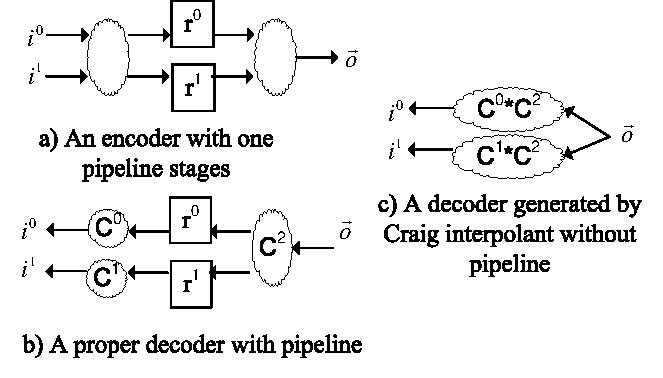
\includegraphics[width=0.5\textwidth]{pipeline}
\end{center}
\caption{The pipelined encoder and its decoders}
  \label{fig_pipe}
\end{figure}

For example,
one simple encoder is shown in Figure \ref{fig_pipe}a).
It has a pipeline stage $\vec{stg}^0$ with some registers.
The inputs variables $\vec{i}$ are used to compute $\vec{stg}^0$,
while $\vec{stg}^0$ are used to compute the output variables $\vec{o}$.
According to this structure,
$\vec{stg}^0$ can be uniquely determined by $\vec{o}$,
while $\vec{i}$ can be uniquely determined by $\vec{stg}^0$.

So,
a properly designed decoder,
often written by human engineers,
should be like the one shown in Figure \ref{fig_pipe}b),
which recovers $\vec{stg}^0$ from $\vec{o}$ with combinational logic $C^1$,
and further recovers $\vec{i}$ from $\vec{stg}^0$ with combinational logic $C^0$.
In such a decoder,
the critical path is cut by registers $\vec{stg}^0$, 
which improves the circuit speed.

% 
% Such a decoder has the following advantages:
% % \begin{enumerate}
% %  \item 
%  \textbf{First},
%  $C^2$ is shared in recovering $i^0$ and $i^1$,
%  which improves the circuit area.
% %  \item 
%  \textbf{Second},
%  the critical path is cut by registers $r^0$ and $r^1$, 
%  which improves the circuit speed.
% %  \item 
% %  \textbf{Finally},
% %  the pipeline structure is preserved,
% %  which makes it much more easier to be understood by human.
% % \end{enumerate}


However,
all complementary synthesis algorithms \cite{ShenTCAD10,ShenTCAD11,ShenTCAD12,LiuICCAD11,LiuTCAD12,TuDAC13}
generate the decoders with Jiang's algorithm \cite{InterpBoolFunction} 
based on Craig interpolant \cite{Craig}.
As shown in Figure \ref{fig_pipe}c),
these decoders recover $\vec{i}$ directly from $\vec{o}$ 
with a large combinational logic $C^0*C^1$.
Such a decoder is unnecessarily slow because 
there are no registers to cut its critical path.

% Thus,
% such decoder have the following major shortcomings:
% % \begin{enumerate}
% %  \item 
%  \textbf{First}, their circuit area are unnecessarily large because 
%  the common logic $C^2$ are hidden deeply in
%  the two large combinational logic $C^0*C^2$ and $C^1*C^2$.
%  It is difficult to factor out $C^2$, 
%  especially for XOR-rich circuits.
% %  \item 
%  \textbf{Second}, the decoder is unnecessarily slow because 
%  there are no registers to cut its critical path.
% %  \item 
% %  \textbf{Finally},the decoder's pipeline structure are lost, 
% %  which make it very difficult to be understood by human engineers.
% % \end{enumerate}

To generate a proper decoder like Figure \ref{fig_pipe}b) in complementary synthesis,
we propose a novel algorithm to first find out the encoder's pipeline registers in each pipeline stage,
and then characterize all Boolean functions that recover each of these pipeline registers
from the next pipeline stage or output variables $\vec{o}$,
and finally characterize the Boolean functions that recover the encoder's input variables 
from the first pipeline stage.

\begin{figure}[t]
\begin{center}
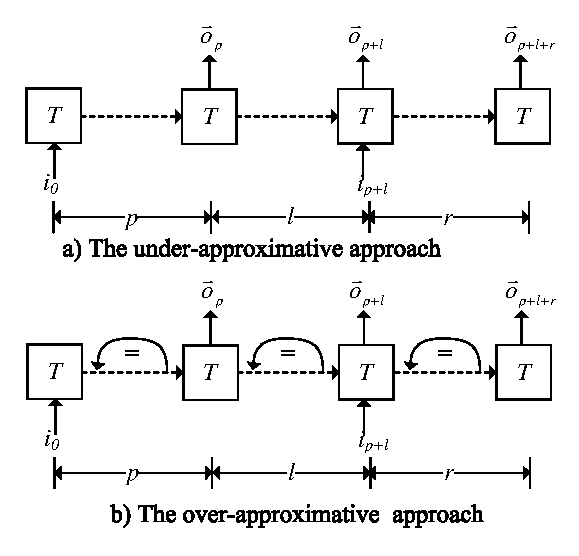
\includegraphics[width=0.5\textwidth]{pcln}
\end{center}
\caption{The under and over-approximative approaches}
  \label{fig_pc}
\end{figure}

Experimental results on several complex encoders,
such as PCI Express \cite{pcie21} and Ethernet \cite{IEEE8023_S4},
indicate that
this algorithm can always correctly generate a pipelined decoder with significantly improved speed.
% and the generated decoder are much more easier to be understood.

\emph{The remainder of this paper is organized as follows}.
%Section \ref{sec_casestudy} explains our ideas with a simple example.
Section \ref{sec_prem} introduces the background material;
Section \ref{sec_pipeinfer} infers the pipeline structure,
while Section \ref{sec_char} characterizes the Boolean functions that recover the input variables and pipeline registers;
Sections \ref{sec_exp} and \ref{sec_relwork} present the experimental results and related works;
Finally,
Section \ref{sec_conclude} sums up the conclusion.


\section{Preliminaries}\label{sec_prem}

% \subsection{Flow control mechanism}\label{subsec_fc}



\subsection{Propositional satisfiability}\label{subsec_SAT}
% We use a denotation similar to that of \cite{TuDAC13}.
The Boolean set is $\mathbb{B}=\{0,1\}$.
A variables vector is $\vec{v}=(v,\dots)$.
The number of variables in $\vec{v}$ is $|\vec{v}|$.
If a variable $v$ is a member of $\vec{v}$,
% that is $\vec{v}=(\dots,v,\dots)$,
then we say $v\in\vec{v}$;
otherwise $v\notin\vec{v}$.
% For a variable $v$ and a vector $\vec{v}$,
% if $v\notin\vec{v}$,
$v\cup\vec{v}$ is the vector containing both $v$ and all members of $\vec{v}$.
$\vec{v}/\vec{w}$ is the vector containing all members of $\vec{v}$ but no member of $\vec{w}$.
% For two vectors $\vec{a}$ and $\vec{b}$,
$\vec{a}\cup\vec{b}$ is the vector with all members of $\vec{a}$ and $\vec{b}$.
The set of truth valuations of $\vec{v}$ is $[\![\vec{v}]\!]$,
for instance,
$[\![(v_1,v_2)]\!]=\{(0,0),(0,1),(1,0),(1,1)\}$.

% A Boolean formula $F$ over a variable set $V$ is constructed by connecting variables from $V$ 
% with symbols $\neg$, $\wedge$, $\vee$ and $\Rightarrow$,
% which stand for logical connectives negation, conjunction, disjunction, and implication, respectively.

The propositional satisfiability problem(SAT) for a formula $F$ over a variable set $V$ 
is to find a satisfying assignment $A:V\to \mathbb{B}$,
so that $F$ can be evaluated to $1$.
If $A$ exists, then $F$ is satisfiable;
otherwise,
it is unsatisfiable.

% A computer program that decides the existence of such a satisfying assignment is called a SAT solver,
%  such as Zchaff\cite{CHAFF},
%  Grasp\cite{grasp},
%  Berkmin\cite{BERKMIN},
%  and MiniSat\cite{EXTSAT}.
 
% Normally,
% a SAT solver requires the formula to be represented in the conjunctive normal form(CNF),
% in which a formula is a conjunction of its clause set,
% and a clause is a disjunction of its literal set,
% and a literal is a variable or its negation.
% A formula in the CNF format is also called a SAT instance,


% \subsection{Cofactoring}\label{subsec_pre_cofact}

% For a Boolean function $f:B^n\to B$,
% we use $supp(f)$ to denote its support set $\{v_1\dots v_n\}$.
% According to \cite{EFFSATUSMCCO},
% the positive and negative cofactors of $f(v_1\dots v\dots v_n)$ with respect to variable
% $v$ are $f_{v\equiv 1}=f(v_1\dots 1\dots v_n)$ and $f_{v\equiv 0}=f(v_1\dots 0\dots v_n)$,
% respectively.
% % Existential quantification of $f(v_1\dots v\dots v_n)$ with respect to a
% % variable $v$ is $\exists v f=f_v+f_v’$.
% \textbf{Cofactoring} is the action that applies 1 or 0 to $v$ to get $f_{v\equiv 1}$ or $f_{v\equiv 0}$.

% \subsection{Craig interpolation}\label{subsec_pre_interp}
% Craig\cite{Craig} had proved the following theorem:
% \begin{theorem}[Craig Interpolation Theorem\cite{Craig}]\label{thm_craig}
For formulas $\phi_A$ and $\phi_B$,
with $\phi_A\wedge \phi_B$ unsatisfiable,
there exists a formula $\phi_I$ referring only
to the common variables of $\phi_A$ and $\phi_B$ such that $\phi_A\Rightarrow \phi_I$
and $\phi_I\wedge \phi_B$ is unsatisfiable.
$\phi_I$ is the \textbf{Craig interpolant} \cite{Craig} of $\phi_A$ with respect to $\phi_B$.
% \end{theorem}
% and can be computed with McMillan's algorithm \cite{InterpBoolFunction}.

% In the remainder of this paper,
% we will focus on the propositional logic only,
% There are many approaches to generate interpolants for propositional logic,
% so please refer to Krajicek\cite{interp_Krajicek},
% Pudlak\cite{interp_Pudlak} and McMillan\cite{interp_McMillan} for more details.
% which is generated by MiniSat\cite{EXTSAT}.


% \subsection{Incremental SAT mechanism of MiniSat solver}\label{subsec_incsat}

% In this paper,
% MiniSat \cite{EXTSAT} is used in this paper to solve all formulas.
% % Like many other SAT solver based on conflict driven learning \cite{CONFLICTLEARN},
% It generates learned clauses from conflicts,
% and records them to prevent the same conflict from rising again.
% % This mechanism can significantly speedup a particular SAT solving.
% % In many applications,
% % there often exists a serial of CNF formulas tightly related to each other.
% % If the learned clauses can be shared between them,
% % then these formulas can be solved much faster.
% It provides an incremental SAT mechanism that can share learned clauses between related formulas
% to solve them faster.
% This mechanism includes two procedures:
% % \begin{enumerate}
% % \item
% $addClause(F)$ used to add a CNF formula $F$ to the clause database, and
% % \item
% $solve(A)$ that solves $F$ with a set of literals $A$ as assumptions
% .
% \end{enumerate}


\subsection{Finite state machine}\label{subsec_fsm}

% \begin{figure}[t]
% \centering
% 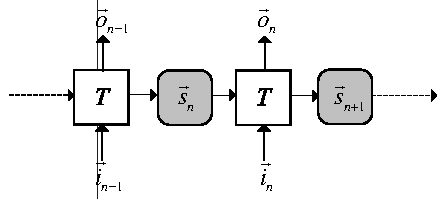
\includegraphics{mealy}
% \caption{Mealy finite state machine}
% \label{mealy}
% \end{figure}

The encoder is modeled by a finite state machine(FSM) $M=(\vec{s},\vec{i},\vec{o},T)$,
consisting of a state variable vector $\vec{s}$,
% an initial state $s_0\in S$,
an input variable vector $\vec{i}$,
% a finite set of configuration letters $C$,
an output variable vector $\vec{o}$,
and a transition function $T: [\![\vec{s}]\!]\times [\![\vec{i}]\!]\to [\![\vec{s}]\!]\times [\![\vec{o}]\!]$ 
that computes the next state and output variable vector from the current state and input variable vector.

% As shown in Figure \ref{mealy},
% as well as in the remainder of this paper,
% the state is represented as a gray round corner box,
% and the transition function $T$ is represented as a white rectangle.
The behavior of FSM $M$ can be reasoned by unrolling transition function for multiple steps.
The state variable $s\in\vec{s}$, input variable $i\in\vec{i}$ and output variable $o\in\vec{o}$ at the $n$-th step 
are respectively denoted as $s_n$, $i_n$ and $o_n$.
Furthermore,
the state, the input and the output variable vectors at the $n$-th step are respectively denoted as $\vec{s}_n$, $\vec{i}_n$ and $\vec{o}_n$.
% We further denote the sequence of state, input letter and output letter from the $n$-th to the $m$-th step respectively as $s_n^m$, $i_n^m$ and $o_n^m$.
A \textbf{path} is a state sequence $<\vec{s}_n,\dots,\vec{s}_m>$ with $\exists \vec{i}_j\vec{o}_j (\vec{s}_{j+1},\vec{o}_j)\equiv T(\vec{s}_j,\vec{i}_j)$ for all $n\le j< m$.
A \textbf{loop} is a path $<\vec{s}_n,\dots,\vec{s}_m>$ with $\vec{s}_n\equiv \vec{s}_m$.

\subsection{The halting algorithm to determine 
if an input variable can be uniquely determined by a bounded sequence of output variable vector}\label{subsec_chkextdec}

% All the state-of-the-art complementary synthesis algorithms 
% [\citeNP{ShenICCAD09};\citeyearNP{ShenTCAD10,ShenTCAD11,ShenTCAD12};\citeNP{LiuICCAD11};\citeyearNP{LiuTCAD12};\citeNP{TuDAC13}] assume that $\vec{i}$ can be uniquely determined,
% so they always take $\vec{i}$ as a whole,
% and never consider individual variables $i\in\vec{i}$.
% But in this paper,
% we need to check each $i\in\vec{i}$ one by one,
% so there may be minor differences between our presentation here and that of 
% [\citeNP{ShenICCAD09};\citeyearNP{ShenTCAD10,ShenTCAD11,ShenTCAD12};\citeNP{LiuICCAD11};\citeyearNP{LiuTCAD12};\citeNP{TuDAC13}].

% What we describe here is a halting algorithm to determine if an input variable 
% can be uniquely determined by a bounded sequence of output variable vector.
The first halting algorithm \cite{ShenTCAD11} iteratively unrolls the transition function.
For each iteration,
it uses an under-approximative and an over-approximative approaches 
presented respectively in \ref{subsub_sound} and \ref{subsub_complete}
to determine the answer.
% The first one is an under-approximative one that presented in \ref{subsub_sound},
% while the second one is an over-approximative one presented in \ref{subsub_complete}.
% That is,
% when the first one says YES then the final answer is YES,
% and when the second approach says NO then the final answer is NO.
We will show in \ref{subsub_algo} that 
these two approaches will eventually converge to a conclusive answer.

\subsubsection{The under-approximative approach}\label{subsub_sound}

As shown in Figure \ref{fig_pc}a),
on the unrolled transition functions,
an input variable $i\in\vec{i}$ can be uniquely determined,
if there exist three integers $p$, $l$ and $r$,
such that for any particular valuation of the output sequence $<\vec{o}_p,\dots,\vec{o}_{p+l+r}>$,
$i_{p+l}$ cannot be 0 and 1 at the same time.
This is equal to the unsatisfiability of $F_{PC}(p,l,r)$ in Equation (\ref{uniqt1}).

\begin{multline}\label{uniqt1}
% \begin{split}
F_{PC}(p,l,r):=\\
\left\{
\begin{array}{cc}
&\bigwedge_{m=0}^{p+l+r}
\{
(\vec{s}_{m+1},\vec{o}_m)\equiv T(\vec{s}_m,\vec{i}_m)
\}
\\
\wedge&\bigwedge_{m=0}^{p+l+r}
\{
(\vec{s'}_{m+1},\vec{o'}_m)\equiv T(\vec{s'}_m,\vec{i'}_m)
\}
\\
\wedge&\bigwedge_{m=p}^{p+l+r}\vec{o}_m\equiv \vec{o'}_m \\
\wedge& i_{p+l}\equiv 1 \wedge  i'_{p+l}\equiv 0 
% \wedge&\bigwedge_{m=0}^{p+l+r}assertion(\vec{i}_m) \\
% \wedge&\bigwedge_{m=0}^{p+l+r}assertion(\vec{i'}_m) 
\end{array}
\right\}
% \end{split}
\end{multline}


% \begin{figure*}[t]
% \begin{center}
% 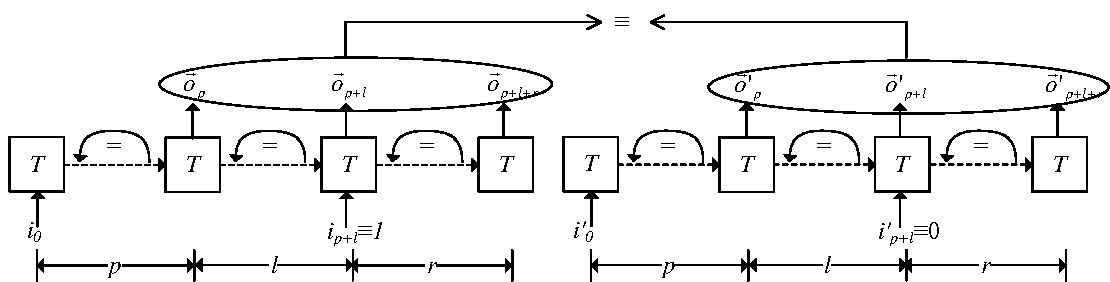
\includegraphics[width=\textwidth]{ln}
% \end{center}
% \caption{The over-approximative  approach checking if $i_{p+l}$ can NOT be uniquely determined}
%   \label{fig_ln}
% \end{figure*}

Here,
$p$ is the length of the prefix state transition sequence.
$l$ and $r$ are the lengths of the two output sequences 
$<\vec{o}_{p+1},\dots,\vec{o}_{p+l}>$ and $<\vec{o}_{p+l+1},\dots,\vec{o}_{p+l+r}>$
used to determine $i_{p+l}$.
Line 2 of Equation (\ref{uniqt1}) corresponds to the path in Figure \ref{fig_pc}a),
while Line 3 is a copy of it.
These two paths are of the same length.
Line 4 forces these two paths' output sequences to be the same,
while Line 5 forces their $i_{p+l}$ to be different.
% Line 5 and 6 are the assertion predicates given 
% by the user that constrain the valid valuation on $\vec{i}$.
% PC in $F_{PC}$ is the abbreviation of "parameterized complementary",
% which means $F_{PC}(p,l,r)$ is used to check whether the encoder's input can be uniquely determined with the three parameters $p$, $l$ and $r$.


% According to Figure \ref{fig_pc},
% the first three lines of Equation (\ref{uniqt1}) are two unrolled transition function sequences with the same output sequences.
% They can always be satisfied with the same input variable vectors and initial state vector.
% And the last two lines are constraints on input variable vectors.
% We always check their satisfiability before running our algorithm.
% So the unsatisfiability of $F_{PC}(p,l,r)$ always means $i_{p+l}\equiv i'_{p+l}$.


% According to Figure \ref{fig_pc},
% % it is obvious that,
% if $F_{PC}(p,l,r)$ is unsatisfiable,
% then $F_{PC}(p',l',r')$ is also unsatisfiable for $p'\ge p$, $l'\ge l$ and $r'\ge r$.
According to Equation (\ref{uniqt1}),
% and Figure \ref{fig_pc},
% we can find that,
for $p'\ge p$, $l'\ge l$ and $r'\ge r$,
the clause set of $F_{PC}(p',l',r')$ is a super set of $F_{PC}(p,l,r)$.
% This also lead to the same conclusion.
% This means,
So,
the bounded proof of $F_{PC}(p,l,r)$'s unsatisfiability
can be generalized to unbounded cases.


\begin{proposition}\label{prop_pc1}
If $F_{PC}(p,l,r)$ is unsatisfiable,
% then $i_{p+l}$ cannot take on two different values for any particular valuation of the output sequence $<\vec{o}_{p},\dots,\vec{o}_{p+l+r}>$,
then $i_{p+l}$ can be uniquely determined by $<\vec{o}_{p},\dots,\vec{o}_{p+l+r}>$ for all larger $p$, $l$ and $r$.
\end{proposition}

% Equation (\ref{uniqt1}) doesn't include an initial state,
% instead it uses the $p$ steps prefix state sequence $<\vec{s_0},\dots,\vec{s_{p-1}}>$ 
% to propagate $assertion(\vec{i})$ into $<\vec{s_p},\dots,\vec{s_{p+l+r}}>$,
% such that some states that can't be reached with $assertion(\vec{i})$ can be eliminated.
% This leads to two major advantages over considering initial states:
% First,
% it simplify and speedup our algorithm by avoiding the need to compute the reachable state set or inductive invariants.
% \cite{TuDAC13} rules out unreachable states by inferring inductive invariants.
% But it can't handle our most complex XFI benchmark \cite{ShenTCAD11},
% while our algorithms always can.
% Second, 
% % and more importantly,
% ignoring initial states improves the decoder's reliability by 
% making the decoder's output depend only on  bounded history of its input.
% Thus any corrupted $\vec{o}$ can only affect the decoder for finite number of steps.
% 
% Of course ignoring initial states has one drawback that it is a little bit too stronger than necessary.
% That is,
% it requires that $\vec{i}$ must be uniquely determined on a larger state set $R^p$ 
% that is reachable in $p$ steps from any states,
% instead of on the smaller state set $R$ that is reachable from initial states.
% In some cases,
% our algorithm may fail to handle properly designed encoders.
% % It is obvious that $R\subset R^p$.
% But this has never happen on all our benchmarks.
% 
% Their work is orthogonal to ours.
% So to simplify our discussion,
% we will not integrate their work here.
% At the same time,
% for all the benchmarks we have tried,
% our current approach is sufficient.



% $d$ is the relative delay between $o_{n+d-l}^{n+d-1}$ and $i_n$,
% while $l$ is the length of $o_{n+d-l}^{n+d-1}$,
% and $p$ is the length of the prefix path used to rule out some unreachable states.
% This condition is formally defined below:

% \begin{definition11}\label{def_pcc}%\addtolength{\itemsep}{-0.5\baselineskip}
% %{\setlength{\baselineskip}{0.5\baselineskip}
% \textbf{Parameterized Complementary Condition (PC)}:
% For encoder $E$,
% assertion $R$,
% and three integers $p$,$d$ and $l$,
% $E\vDash PC(p,d,l,R)$ holds if
% \begin{enumerate}
%  \item $i_n$ can be uniquely determined by $o_{n+d-l}^{n+d-1}$ on $s_{n-p}^{n+d-1}$.
%  \item $R$ covers all $c_x$, where $n-p\le x\le n+d-1$.
% \end{enumerate}
% 
% This equals the unsatisfiability of $F_{PC}(p,d,l,R)$ in Equation (\ref{uniqt1}).
% We further define $E\vDash PC(R)$ as $\exists p,d,l:E\vDash PC(p,d,l,R)$.
% \end{definition11}

%This definition is the same as that of Subsection \ref{subsec_chkextdec} and paper \cite{ShengYuShen:iccad09}.


% At the same time,
% the last three lines of Equation (\ref{uniqt1}) correspond to Condition 2 of Definition \ref{def_pcc}.
% The 6th and the 7th lines constrain that all configuration letters are equal to $c$,
% while the last line constrains $c$ to be covered by $R$.

% The algorithm based on checking $E\vDash PC(R)$\cite{ShengYuShen:iccad09,ShengYuShen:tcad} just enumerates all combinations of $p$,$d$ and $l$,
% from small to large,
% until $F_{PC}(p,d,l,R)$ becomes unsatisfiable,
% which means that the decoder $E^{-1}$ exists.
% 
% \begin{figure}[b]
% \begin{center}
% 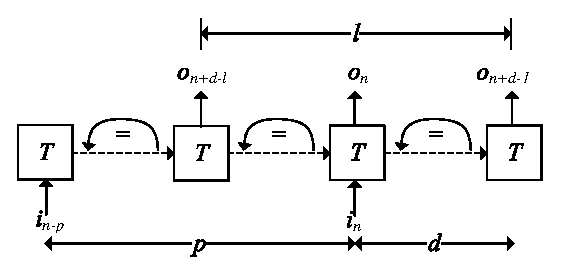
\includegraphics[width=0.45\textwidth]{doubleloop}
% \end{center}
% \caption{The loop-like non-complementary condition}
%   \label{fig_double_loop}
% \end{figure}

\subsubsection{The over-approximative approach}\label{subsub_complete}

If $F_{PC}(p,l,r)$ presented in the last subsection is satisfiable,
there are two possibilities:
\begin{enumerate}
 \item 
$i_{p+l}$ can be uniquely determined by $<\vec{o}_{p},\dots,\vec{o}_{p+l+r}>$ for some larger $p$, $l$ and $r$;
 \item 
$i_{p+l}$ can't be uniquely determined by $<\vec{o}_{p},\dots,\vec{o}_{p+l+r}>$ for any $p$, $l$ and $r$ at all.
\end{enumerate}

If it is the 1st case,
then by iteratively increasing  $p$, $l$ and $r$,
$F_{PC}(p,l,r)$ will eventually become unsatisfiable.
But if it is the 2nd case,
this method will never terminate.

\begin{algorithm}[t]
\SetAlgoVlined
\KwIn{The input variable $i\in\vec{i}$.}
\KwOut{whether $i\in\vec{i}$ can be uniquely determined by $\vec{o}$, and the value of $p$, $l$ and $r$.}
$p$:= 0; ~$l$:= 0;~$r$:= 0\;
\While{$1$}{
   $p$++;~$l$++;~$r$++\;\ShowLnLabel{linepc1}
   \uIf{$F_{PC}(p,l,r)$ is unsatisfiable}{
    \KwRet ($1$, $p$, $l$, $r$);
   }\ShowLnLabel{lnsat}\uElseIf{$F_{LN}(p,l,r)$ is satisfiable} {
    \KwRet ($0$, $p$, $l$, $r$);
   }
}
\caption{$CheckUniqueness(i)$: The halting algorithm to determine 
whether $i\in\vec{i}$ can be uniquely determined by a bounded sequence of output variable vector $\vec{o}$}
\label{alg_pcln}
\end{algorithm}

So,
to obtain a halting algorithm,
we need to distinguish these two cases.
One such solution is shown in Figure \ref{fig_pc}b),
which is similar to Figure \ref{fig_pc}a) but with three additional constraints used to detect loops 
on the three state sequences $<\vec{s}_{0},\dots,\vec{s}_{p}>$,$<\vec{s}_{p+1},\dots,\vec{s}_{p+l}>$ and 
$<\vec{s}_{p+l+1},\dots,\vec{s}_{p+l+r}>$.
It is formally defined in Equation (\ref{uniqln}) with the last three lines corresponding to the three new constraints used to detect loops.

\begin{multline}\label{uniqln}
% \begin{split}
F_{LN}(p,l,r):=\\
\left\{
\begin{array}{cc}
&F_{PC}(p,l,r)\\
\wedge&\bigvee_{x=0}^{p-1}\bigvee_{y=x+1}^{p} \{\vec{s}_x\equiv \vec{s}_y\wedge \vec{s'}_x\equiv \vec{s'}_y\} \\
\wedge&\bigvee_{x=p+1}^{p+l-1}\bigvee_{y=x+1}^{p+l} \{\vec{s}_x\equiv \vec{s}_y\wedge \vec{s'}_x\equiv \vec{s'}_y\} \\
\wedge&\bigvee_{x=p+l+1}^{p+l+r-1}\bigvee_{y=x+1}^{p+l+r} \{\vec{s}_x\equiv \vec{s}_y\wedge \vec{s'}_x\equiv \vec{s'}_y\}
\end{array}
\right\}
% \end{split}
\end{multline}

% LN in $F_{LN}$ stands for "loop non-complementary",
% which means $F_{LN}(p,l,r)$ with three loops is used to check whether 
% the input variable can NOT be uniquely determined.


When $F_{LN}(p,l,r)$ is satisfiable,
then $i_{p+l}$ can't be uniquely determined by $<\vec{o}_{p},\dots,\vec{o}_{p+l+r}>$.
More importantly,
by unrolling these three loops,
we can generalize the satisfiability of $F_{LN}(p,l,r)$ to all larger $p$, $l$ and $r$.
This means:


\begin{proposition}\label{prop_ln1}
If $F_{LN}(p,l,r)$ is satisfiable,
then $i_{p+l}$ cannot be uniquely determined by $<\vec{o}_{p},\dots,\vec{o}_{p+l+r}>$ for all larger $p$, $l$ and $r$.
\end{proposition}

Please refer to \cite{ShenTCAD11} for more detail of this.

\subsubsection{The full algorithm}\label{subsub_algo}

With Propositions \ref{prop_pc1} and \ref{prop_ln1},
we can generalize their bounded proof to unbounded cases.
This leads to the halting
Algorithm \ref{alg_pcln} that search for $p$, $l$ and $r$ that enable
an input variable $i_{p+l}$ to be uniquely determined by the output sequence $<\vec{o}_{p},\dots,\vec{o}_{p+l+r}>$:
\begin{enumerate}
 \item 
On the one hand, 
if there exists such $p$, $l$ and $r$,
then let $p':=max(p,l,r)$, $l':=max(p,l,r)$ and $r':=max(p,l,r)$.
From Propositions \ref{prop_pc1},
we know that $F_{PC}(p',l',r')$ is unsatisfiable.
So eventually $F_{PC}(p,l,r)$ will become unsatisfiable in Line \ref{linepc1};
 \item
On the other hand,
if there doesn't exist such $p$, $l$ and $r$,
then eventually $p$, $l$ and $r$ will be larger than the encoder's longest path without loop,
which means that there will be three loops in $<\vec{s}_{0},\dots,\vec{s}_{p}>$,$<\vec{s}_{p+1},\dots,\vec{s}_{p+l}>$ and 
$<\vec{s}_{p+l+1},\dots,\vec{s}_{p+l+r}>$.
This will make $F_{LN}(p,l,r)$ satisfiable in Line \ref{lnsat}.
\end{enumerate}

Both cases will lead to this Algorithm's termination.
Please refer to \cite{ShenTCAD11} for more detail of this algorithm's correctness and termination proof.





\section{Inferring the encoder's pipeline structure}\label{sec_pipeinfer}

\subsection{A general model for the encoder}
As shown in Figure \ref{fig_pipeenc},
we assume that the 
the encoder have $n$ pipeline stages.
If we take the combinational logic block $C^j$ as a function,
then this encoder can be represented by the following equations.

\begin{equation}\label{equ_genpipe}
\begin{array}{cccc}
\vec{stg}^0   & := & C^0(\vec{i})         &\\
\vec{stg}^j   & := & C^j(\vec{stg}^{j-1}) & 1\le j\le n-1\\
\vec{o}       & := & C^n(\vec{stg}^{n-1}) &
\end{array}
\end{equation}


\begin{figure}[b]
\begin{center}
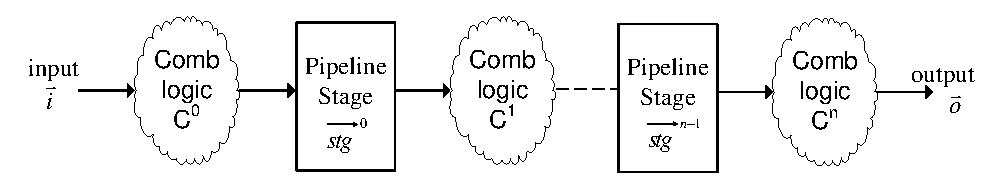
\includegraphics[width=0.5\textwidth]{pipemod}
\end{center}
\caption{A general structure of the encoder}
  \label{fig_pipeenc}
\end{figure}


Thus,
each $C^j$ can be seen as a small encoder that computes $\vec{stg}^j$ or $\vec{o}$
from $\vec{stg}^{j-1}$ or $\vec{i}$.

In the remainder of this paper,
superscript always means the pipeline stage,
while the subscript,
as mentioned in Subsection \ref{subsec_fsm},
always means the step index in the unrolled transition function.
For example,
$\vec{stg}^j$ is the $j$-th pipeline stage.
While $\vec{stg}^j_i$ is the value of this $j$-th pipeline stage 
at the $i$-th step in the unrolled state transition function.

\subsection{Inferring $p$, $l$ and $r$}\label{subsec_inferplr}
Before inferring the pipeline stages,
we first apply Algorithm \ref{alg_pcln} to infer the value of $p$, $l$ and $r$ that can make the 
output sequence $<o_{p},\dots,o_{p+l+r}>$ uniquely determine all $i_{p+l}\in \vec{i}_{p+l}$.

As there are more than one $i\in \vec{i}$,
we need to apply Algorithm \ref{alg_pcln} for each $i\in \vec{i}$ 
to get the $p$, $l$ and $r$ for each of them.

And then we set the final $p$,$l$ and $r$ to be the maximal $p$, $l$ and $r$ of all $i\in \vec{i}$ respectively.
According to Equation \ref{uniqt1},
these values of $p$, $l$ and $r$ can indeed make the 
output sequence $<o_{p},\dots,o_{p+l+r}>$ uniquely determine all $i_{p+l}\in \vec{i}_{p+l}$.


\subsection{Minimizing $r$ and $l$}\label{reduceing}

\begin{algorithm}[t]
\SetAlgoVlined
\For{$r':=r \to 0$} {
\ShowLnLabel{testr_1}
  \If{$r'\equiv 0$ or $F_{PC}(p,l,r'-1)$ is satisfiable for some $i\in \vec{i}$} {
    break
  }
}
return $r'$
\caption{$RemoveRedundancy(p,l,r)$}
\label{algo_remove2}
\end{algorithm}

As Algorithm \ref{alg_pcln} increases $p$, $l$ and $r$ simultaneously,
there may be some redundancy in the value of $l$ and $r$.
So we need to first minimize $r$ in Algorithm \ref{algo_remove2}


% To simplify the presentation,
% we will only introduce the $r$ case.
In Line \ref{testr_1},
when $F_{PC}(p,l,r'-1)$ is satisfiable,
then $r'$ is the last one that makes it unsatisfiable,
we return it directly.
On the other hand,
when $r'\equiv 0$,
$F_{PC}(p,l,0)$ must have been tested in the last iteration,
and the result must be unsatisfiable.
In this case we return $0$.

% Minimizing $l$ is similar but with two exceptions:
% First, 
% the range of $l'$ to be enumerated contains some negative value,
% which means $i$ only depend on the value of $o$ in the future.
% Second,
% to be compatible with such cases,
% we use a new formula $F'_{PC}$ in Line \ref{testr_2}.
% When $l\ge 0$,
% $F'_{PC}$ equals to $F_{PC}$.
% But when $l<0$,
% $F'_{PC}$ is define below:
% 
% \begin{multline}\label{uniqt11}
% % \begin{split}
% F'_{PC}(p,l,r):=\\
% \left\{
% \begin{array}{cc}
% &\bigwedge_{m=0}^{p+l+r}
% \{
% (\vec{s}_{m+1},\vec{o}_m)\equiv T(\vec{s}_m,\vec{i}_m)
% \}
% \\
% \wedge&\bigwedge_{m=0}^{p+l+r}
% \{
% (\vec{s'}_{m+1},\vec{o'}_m)\equiv T(\vec{s'}_m,\vec{i'}_m)
% \}
% \\
% \wedge&\bigwedge_{m=p-l}^{p+r}\vec{o}_m\equiv \vec{o'}_m \\
% \wedge& i_{p}\equiv 1 \wedge  i'_{p}\equiv 0 
% % \wedge&\bigwedge_{m=0}^{p+l+r}assertion(\vec{i}_m) \\
% % \wedge&\bigwedge_{m=0}^{p+l+r}assertion(\vec{i'}_m) 
% \end{array}
% \right\}
% % \end{split}
% \end{multline}
% 
% The only change of Equation (\ref{uniqt11}) compared to Equation (\ref{uniqt1})
% are that 
% the range of output vector is change to $p-l\le m\le p+r$,
% while the subscripts of $i$ and $i'$ in the last line refer to $p$ only,
% $l$ are removed.

Now, 
we have a minimized $r$ from Algorithm \ref{algo_remove2},
which can make $\vec{i}_{p+l}$ to be uniquely determined by $<\vec{o}_{p},\dots,\vec{o}_{p+l+r}>$.

We further require that 
\begin{enumerate}
 \item As shown in Figure \ref{fig_pc1},
 $l$ can be reduced to 0,
 which means $\vec{i}_{p}$ can be uniquely determined by $<\vec{o}_{p},\dots,\vec{o}_{p+r}>$,
 that is,
 the set of future outputs.
 \item The above mentioned output sequence $<\vec{o}_{p},\dots,\vec{o}_{p+r}>$ 
 can be further reduced to $\vec{o}_{p+r}$.
 This means $\vec{o}_{p+r}$ is the only output vector needed to recover the input vector $\vec{i}_p$.
\end{enumerate}

Checking these two requirements
equals to checking the unsatisfiability of the following equation.

\begin{multline}\label{uniqt11}
% \begin{split}
F'_{PC}(p,r):=\\
\left\{
\begin{array}{cc}
&\bigwedge_{m=0}^{p+r}
\{
(\vec{s}_{m+1},\vec{o}_m)\equiv T(\vec{s}_m,\vec{i}_m)
\}
\\
\wedge&\bigwedge_{m=0}^{p+r}
\{
(\vec{s'}_{m+1},\vec{o'}_m)\equiv T(\vec{s'}_m,\vec{i'}_m)
\}
\\
\wedge&\vec{o}_{p+r}\equiv \vec{o'}_{p+r} \\
\wedge& i_{p}\equiv 1 \wedge  i'_{p}\equiv 0 
% \wedge&\bigwedge_{m=0}^{p+l+r}assertion(\vec{i}_m) \\
% \wedge&\bigwedge_{m=0}^{p+l+r}assertion(\vec{i'}_m) 
\end{array}
\right\}
% \end{split}
\end{multline}


This equation seems much stronger than the general requirement in Equation (\ref{uniqt1}).
But we will show in experimental results that 
they are always fulfilled.

\begin{figure}[t]
\begin{center}
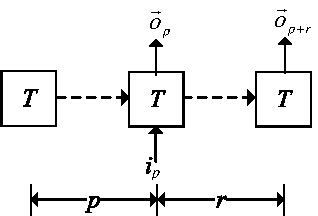
\includegraphics[width=0.25\textwidth]{pc1}
\end{center}
\caption{Recovering input with reduced output sequence}
  \label{fig_pc1}
\end{figure}

\subsection{Inferring pipeline stages}\label{subsec_inferstage}

Now,
with the inferred $p$ and $r$,
we need to generalize $F'_{PC}$ in Equation (\ref{uniqt11}) to the following new formula that
can determine whether a particular variable $v$ at step $j$
can be uniquely determined by a vector $\vec{w}$ at step $k$.
Now $v$ and $\vec{w}$ can be either input, registers or output variables.

\begin{multline}\label{uniqt2}
% \begin{split}
F''_{PC}(p,r,v,j,\vec{w},k):=\\
\left\{
\begin{array}{cc}
&\bigwedge_{m=0}^{p+r}
\{
(\vec{s}_{m+1},\vec{o}_m)\equiv T(\vec{s}_m,\vec{i}_m)
\}
\\
\wedge&\bigwedge_{m=0}^{p+r}
\{
(\vec{s'}_{m+1},\vec{o'}_m)\equiv T(\vec{s'}_m,\vec{i'}_m)
\}
\\
\wedge&\vec{w}_{k}\equiv \vec{w'}_{k} \\
\wedge& v_{j}\equiv 1 \wedge  v'_{j}\equiv 0 
% \wedge&\bigwedge_{m=0}^{p+l+r}assertion(\vec{i}_m) \\
% \wedge&\bigwedge_{m=0}^{p+l+r}assertion(\vec{i'}_m) 
\end{array}
\right\}
% \end{split}
\end{multline}

Obviously,
when $F''_{PC}(p,r,v,j,\vec{w},k)$ is unsatisfiable,
$\vec{w}_k$ can uniquely determine $v_j$.

The last pipeline stage $\vec{stg}^{n-1}$ is 
exactly the set of registers $s\in \vec{s}$ 
that can be uniquely determined at the $p+r$-th step by $\vec{o}$.
% With Equation (\ref{uniqt2}),
It can be formally defined as:

\begin{multline}\label{stgn_1}
 \vec{stg}^{n-1} := 
\left\{
 s\in \vec{s} ~| 
\begin{array}{cc}
 F''_{PC}(p,r,
 s,p+r,
 \vec{o},p+r)\\
 ~is~unsatisfiable
\end{array}
\right\}
\end{multline}

% And the second to last pipeline stage $\vec{stg}^{n-2}$ 
% is exactly the set of registers $s\in \vec{s}/\vec{stg}^{n-1}$
% that can be uniquely determined at the $p+r-1$-th step by $\vec{stg}^{n-1}$ at $p+r$-th step.
% 
% \begin{multline}\label{stgn_2}
%  \vec{stg}^{n-2} := \\
%  \left\{
%  s\in \vec{s}/\vec{stg}^{n-1} ~| 
% \begin{array}{cc}
%  F''_{PC}(p,r,s,p+r-1,\vec{stg}^{n-1},p+r)\\
%  ~is~unsatisfiable
% \end{array}
% \right\}
% \end{multline}

Similarly,
for $0\le j\le n-2$,
$\vec{stg}^j$ at $j-((n-2)-(p+r-1))$-th step
can be uniquely determined by $\vec{stg}^{j+1}$ at $j-((n-2)-(p+r-1))+1$-th step.
So we can recursively defined $\vec{stg}^j$ as :

\begin{multline}\label{stgn_def}
\begin{array}{ccc}
S             & := & \vec{s}/\bigcup_{j<k\le n-2}\vec{stg}^{k}\\
D             & := & (n-2)-(p+r-1)\\
\end{array}
\end{multline}

\begin{multline}\label{stgn_j}
\vec{stg}^{j} := \\
 \left\{
 s\in S ~| 
\begin{array}{cc}
 F''_{PC}(p,r,s,j-D,\vec{stg}^{j+1},j-D+1)\\
 ~is~unsatisfiable
\end{array}
\right\}
\end{multline}

With Equation (\ref{stgn_1}) and (\ref{stgn_j}),
all the pipeline stages can now be inferred.

\subsection{Inferring the pipeline stage that uniquely determines input vector}\label{subsec_inferinput}

According to Figure \ref{fig_pipeenc},
$\vec{stg}^0$ defined in Equation (\ref{stgn_j}) is
exactly the pipeline stage that uniquely determined the input vector $\vec{i}$.

But in real encoders,
this may not be the case.
So we need to search for the smallest $j$ from $0$ to $n-1$ that can make $\vec{i}$ to be uniquely determined by $\vec{stg}^j$,
that is,
the smallest $j$ that can make $F''_{PC}(p,r,i,p,\vec{stg}^{j},j-D)$ unsatisfiable for all $i\in \vec{i}$,
with $D$ defined in Equation (\ref{stgn_def}).

\section{Characterizing the Boolean function of input variables and pipeline registers}\label{sec_char}
\subsection{Characterizing the Boolean function of the last pipeline stage}

According to Equation (\ref{stgn_1}),
every registers $s\in \vec{stg}^{n-1}$ can be uniquely determined by $\vec{o}$ at the $p+r$-th step,
that is,
$F''_{PC}(p,r,s,p+r,\vec{o},p+r)$ is unsatisfiable and can be partitioned into :

\begin{multline}
 \phi_A := \\
 \left\{
\begin{array}{cc}
&\bigwedge_{m=0}^{p+r}
\{
(\vec{s}_{m+1},\vec{o}_m)\equiv T(\vec{s}_m,\vec{i}_m)
\}
\\
\wedge& s_{p+r}\equiv 1 
\end{array}
\right\}
\end{multline}

\begin{multline}
% \begin{split}
\phi_B := \\
\left\{
\begin{array}{cc}
&\bigwedge_{m=0}^{p+r}
\{
(\vec{s'}_{m+1},\vec{o'}_m)\equiv T(\vec{s'}_m,\vec{i'}_m)
\}
\\
\wedge&\vec{o}_{p+r}\equiv \vec{o'}_{p+r} \\
\wedge& s'_{p+r}\equiv 0 
% \wedge&\bigwedge_{m=0}^{p+l+r}assertion(\vec{i}_m) \\
% \wedge&\bigwedge_{m=0}^{p+l+r}assertion(\vec{i'}_m) 
\end{array}
\right\}
% \end{split}
\end{multline}

As $F''_{PC}(p,r,s,p+r,\vec{o},p+r)$ equals to $\phi_A \wedge \phi_B$,
so $\phi_A \wedge \phi_B$ is unsatisfiable.
And the common variables of $\phi_A$ and $\phi_B$ is $\vec{o}_{p+r}$.

According to \cite{InterpBoolFunction},
a Craig interpolant $\phi_I$ of $\phi_A$ with respect to $\phi_B$ can be constructed,
which refer only to $\vec{o}_{p+r}$,
and covers all the valuation of $\vec{o}_{p+r}$ that can make $s_{p+r}\equiv 1$.
At the same time,
$\phi_I\wedge \phi_B$ is unsatisfiable,
which means $\phi_I$ covers nothing that can make $s_{p+r}\equiv 0$.

Thus,
$\phi_I$ can be used as the decoder's Boolean function that recovers $s\in \vec{stg}^{n-1}$ from $\vec{o}$.

\subsection{Characterizing the Boolean function of the other pipeline stages}
Similar to last subsection,
we can partition the unsatisfiable formula $F''_{PC}(p,r,s,j-D,\vec{stg}^{j+1},j-D+1)$ 
in Equation (\ref{stgn_j}) into the following two equations:

\begin{multline}
 \phi_A := \\
 \left\{
\begin{array}{cc}
&\bigwedge_{m=0}^{p+r}
\{
(\vec{s}_{m+1},\vec{o}_m)\equiv T(\vec{s}_m,\vec{i}_m)
\}
\\
\wedge& s_{j-D}\equiv 1 
\end{array}
\right\}
\end{multline}

\begin{multline}
% \begin{split}
\phi_B := \\
\left\{
\begin{array}{cc}
&\bigwedge_{m=0}^{p+r}
\{
(\vec{s'}_{m+1},\vec{o'}_m)\equiv T(\vec{s'}_m,\vec{i'}_m)
\}
\\
\wedge&\vec{stg}^{j+1}_{j-D+1}\equiv \vec{stg'}^{j+1}_{j-D+1} \\
\wedge& s'_{j-D}\equiv 0 
% \wedge&\bigwedge_{m=0}^{p+l+r}assertion(\vec{i}_m) \\
% \wedge&\bigwedge_{m=0}^{p+l+r}assertion(\vec{i'}_m) 
\end{array}
\right\}
% \end{split}
\end{multline}

Again,
a Craig interpolant $\phi_I$ of $\phi_A$ with respect to $\phi_B$ can be constructed,
and used as the decoder's Boolean function that recovers $s\in \vec{stg}^{j}$ from $\vec{stg}^{j+1}$.

\subsection{Characterizing the Boolean function of the encoder's input variables}

According to Subsection \ref{sec_pipeinfer}.\ref{subsec_inferinput},
we have found the smallest $j$ that can make $F''_{PC}(p,r,i,p,\vec{stg}^{j},j-D)$ unsatisfiable for all $in\in \vec{i}$,
with $D$ defined in Equation (\ref{stgn_def}).
$F''_{PC}(p,r,i,p,\vec{stg}^{j},j-D)$ is unsatisfiable and can be partitioned into :

\begin{multline}
% \begin{split}
\phi_A:=\\
\left\{
\begin{array}{cc}
&\bigwedge_{m=0}^{p+r}
\{
(\vec{s}_{m+1},\vec{o}_m)\equiv T(\vec{s}_m,\vec{i}_m)
\}
\\
\wedge& i_{p}\equiv 1 
% \wedge&\bigwedge_{m=0}^{p+l+r}assertion(\vec{i}_m) \\
% \wedge&\bigwedge_{m=0}^{p+l+r}assertion(\vec{i'}_m) 
\end{array}
\right\}
% \end{split}
\end{multline}

\begin{multline}
% \begin{split}
\phi_B:=\\
\left\{
\begin{array}{cc}
&\bigwedge_{m=0}^{p+r}
\{
(\vec{s'}_{m+1},\vec{o'}_m)\equiv T(\vec{s'}_m,\vec{i'}_m)
\}
\\
\wedge&\vec{stg}^j_{j-D}\equiv \vec{stg'}^j_{j-D} \\
\wedge& i'_{p}\equiv 0 
% \wedge&\bigwedge_{m=0}^{p+l+r}assertion(\vec{i}_m) \\
% \wedge&\bigwedge_{m=0}^{p+l+r}assertion(\vec{i'}_m) 
\end{array}
\right\}
% \end{split}
\end{multline}

Similar to last subsection,
the Craig interpolant $\phi_I$ of $\phi_A$ with respect to $\phi_B$ 
can be used as the decoder's Boolean function that recovers $i\in\vec{i}$ from $\vec{stg}^j$.

\section{Experimental Results}\label{sec_exp}
We have implemented these algorithms in OCaml language,
and solved the generated CNF formulas with MiniSat 1.14 \cite{EXTSAT}.
All experiments have been run on a server with 16 Intel Xeon E5648 processors at 2.67GHz, 
192GB memory, and CentOS 5.4 Linux.
% All these experimental results and programs can be downloaded 
% from https://github.com/shengyushen/compsyn.

% \subsection{Benchmarks}
%  shows all benchmarks used in this paper.
% They come from \cite{ShenTCAD12}.
%  \item The benchmark package sent to us by Liu, the author of \cite{LiuTCAD12}.
%  So there may be some overlap between (2) and (3).
% \end{enumerate}

Table \ref{tab_bench} shows the benchmarks used in this paper.
% They are listed in the order of circuit area.
The 2nd to 3rd column show respectively the number of inputs, outputs and registers of each benchmark.
The area column shows the area of the encoder when mapped to LSI10K library with Design Compiler.
% We use Design compiler here instead of ABC \cite{ABC} used by other researchers 
% because ABC can not read in verilog files with registers generated by our algorithms.
In this paper, 
all area and delay are obtained in the same setting.
% we can compare them to that of \cite{LiuTCAD12}.



\begin{table}[t]
\caption{Benchmarks}
\begin{tabular}{|c|c|c|c|c|}
\hline
 Names     &    \#   &   \#reg &Circuit& Description                         \\
           & in/out  &         &area  &   of Encoders                        \\\hline\hline
 pcie      & 10/11   & 23      & 326  &PCIE 2.0 \cite{pcie21}                               \\
           &         &         &      &                         \\\hline
 xgxs      & 10/10   & 16      & 453  &10Gb Ethernet                \\
           &         &         &      & clause 48 \cite{IEEE8023_S4}             \\\hline
 t2eth     & 14/14   & 49      & 2252 &1Gb Ethernet                    \\
           &         &         &      & clause 36 \cite{IEEE8023_S4}               \\\hline
scram-     &64/64    & 58      & 1034 & inserting 01                  \\
bler       &         &         &      &  flipping             \\\hline
 xfi       & 72/66   & 72      & 7772 &10Gb Ethernet                \\
           &         &         &      & clause 49 \cite{IEEE8023_S4}             \\\hline
\end{tabular}\label{tab_bench}
\end{table}


Table \ref{tab_res} compares the old algorithm from \cite{ShenTCAD11} to this paper's algorithm.
The 2-th to 4-th columns show respectively the run time of \cite{ShenTCAD11}'s algorithm to generate the decoder without pipeline,
and the delay and area of the generated decoder.
While the 5-th to 7-th columns show respectively the run time of this paper's algorithm to generate the pipelined decoder,
and the delay and area of the generated decoder.
The last column shows the number of registers in each pipeline stage.

Comparing the 3rd and the 6-th column indicates that
the decoders' delay have been significantly improved.
And the the last column shows that there actually exist very deep pipeline,
especially the t2eth with 4 pipeline stages.

One thing that is a little bit surprise is,
the two largest benchmarks scrambler and xfi do not have pipeline stages inside.
We study their code and confirm that they actually don't have such pipeline stages.
Their area are so large because they use much wider datapaths with 64 to 72 bits.
% Please refer to IEEE 802.3ae clause 49 \cite{IEEE8023_S4}  for more details.

\section{RELATED PUBLICATIONS}\label{sec_relwork}
%\subsection{Complementary Synthesis}
%%Complementary synthesis is an emerging new research topic,
%%there are only two papers that discuss this problem.
%
%The concept of complementary synthesis was first proposed by us\cite{ShengYuShen:iccad09} in ICCAD 2009.
%Its major shortcomings are that it is incomplete,
%and its run-time overhead of building decoder is too large.
%
%The incomplete problem has been addressed by \cite{ShengYuShen:fmcad10}, while \cite{ShengYuShen:tcad} addresses the second shortcoming by simplifying the SAT instance with unsatisfiable core extraction before building decoders.

% \subsection{Complementary synthesis}\label{subsec_compsyn_relat}
The first complementary synthesis algorithm was proposed by Shen et al.\cite{ShenICCAD09}.
It checks the decoder's existence by iteratively increasing the bound of unrolled transition function sequence,
and generates the decoder's Boolean function by enumerating all satisfying assignments of the decoder's output.
But this algorithm may not halt and is too slow in building the decoder.

The halting problem was independently tackled in Shen et al.\cite{ShenTCAD11} and Liu at al.\cite{LiuICCAD11} by searching for loops in the state sequence,
while the runtime overhead problem was addressed in \cite{ShenTCAD12,LiuICCAD11} by interpolant \cite{InterpBoolFunction}.

Shen et al. \cite{ShenTCAD12} inferred an assertion for configuration pins
that can lead to the decoder's existence.
% It can be seen as a special case of Algorithm \ref{algo_infer},
% with the restriction that the inferred assertion must hold on all steps.
% % to prevent the encoder from leaving the unique state set.
% Our Algorithm \ref{algo_infer},
% on the other hand,
% is the first algorithm that allows states with and without the inferred assertion to be interleaved freely with each other.
% which make it possible to handle encoder with flow control mechanism.
Tu et al.\cite{TuDAC13} proposed a breakthrough algorithm that 
use the encoder's infinite history to generate the decoder's output.
% This algorithm can handle some encoders that cannot be handled by the state-of-the-art algorithms.
% Their work is orthogonal to ours.

% \subsection{Program inversion}\label{subsec_proinv}
% % According to \cite{dim_syn},
% Program inversion derives a program $P^{-1}$
% that negates the computation of a given program $P$.
% So
% it is very similar to complementary synthesis.
% 
% The initial work on program inversion \cite{prog_inv} used proof-based approaches,
% which could handle only very small programs and very simple syntax structures.
% 
% \cite{mtd_autoProginv} inverted first-order functional programs
% by eliminating nondeterminism with LR-based parsing methods.
% But
% the use of functional languages in that work is incompatible with our complementary synthesis.
% 
% \cite{program_inversion_11} assumed that an inverse program was related to the original program,
% so the space of possible inversions can be inferred by automatically
% mining the original program for expressions, predicates, and control flow.
% This algorithm inductively rules out invalid paths that can't fulfill the requirement of inversion
% % to narrow down the space of candidate programs 
% until only the valid ones remain.
% So,
% it can't guarantee the correctness of its solution if its assumptions don't hold.

% \subsection{The completeness of bounded model checking}\label{subsec_bmc_relate}
% Bounded model checking(BMC) \cite{bmc_tacas99} is a model checking technology that considers only paths of limited length.
% So it is an incomplete algorithm.
% Many researchers have tried to find complete approaches for BMC.
% 
% One line of research\cite{bmc_tacas99,RecDiam} tried to find out a bound $b$,
% which can guarantee the correctness of a specification,
% if the specification is correct on all paths that are shorter than $b$.
% Line 8 of Algorithm \ref{algo_infer} finds out the value of $p$,$d$ and $l$ that can prove the non-existence of the decoder,
% which is similar to \cite{bmc_tacas99,RecDiam}.
% 
% The other line of research\cite{kind_tacas99} tried to find a bound for induction,
% such that the correctness of a specification within any bound $b$ implies the correctness on bound $b+1$.
% Our algorithm proves the non-existence of the decoder by unfolding loops.
% This is similar to finding induction patterns \cite{kind_tacas99}.

% \textbf{This paper achieves completeness without following these two approaches.
% Instead,
% it defines two complement uniqueness conditions,
% $LP$ and $LL$,
% and find out proper algorithms to check them.}

%\subsection{Temporal Logic Synthesis}
%%Automatically synthesis of program from logic specification is first identified as Church's problem in 1962\cite{LOGARTHAUTO}.
%%Some early researches \cite{SLVSQFSS,AUTOINF} solve this problem by reducing it to checking emptiness of tree automata.
%
%The temporal logic synthesis was first addressed by Clarke et al.\cite{DSGSYNTMPLG} and Manna et al. \cite{SYNTMPLGSPC}.
%But Pnueli et al. \cite{SYNRCTVMD} pointed out that the complexity of LTL synthesis is double exponent.
%%This high complexity drives researchers turning their focus to find smaller but still useful subset of temporal logic,
%%such that synthesis problem can be solved with lower complexity.
%
%One line of research \cite{CNTLSYNTMDAUTO,DTMGENGMELTL,SYNRCTVDES} focuses on the so-called generalized reactive formulas of the form:
%$(\square \lozenge p_1 \wedge \cdots \square \lozenge p_m) \to (\square \lozenge q_1 \wedge \cdots \square \lozenge q_n)$.
%Complexity of solving synthesis problem for such formula is $O(N^3)$.
%
%The other line of research focuses on finding efficient algorithm \cite{SYNCNTLBNDRPN}
%for expensive safra determination algorithm \cite{CMPLXAUTO} on an useful formula subset,
%or just avoiding it\cite{NEWALGSTRGSYN}.
%
%%Yet another approach is antichain\cite{ANTICHAIN},
%%which reduces the expensive state set computation to computation on maximal and minimal elements of lattice.
%
%Based on these research works,
%some tools\cite{ANZU} that can handle small temporal formulas have been developed.
%
%All these works assume a hostile environment,
%which seems too restrictive for many applications.
%So Fisman et al. \cite{rationalsyn_tacas10}, Chatterjee et al. \cite{assguasyn_tacas07} and Ummels et al. \cite{ralgame_istta06} proposed rational synthesis algorithm,
%which assumes that each agents act to achieve their own goals instead of failing each other.


% \subsection{Protocol converter synthesis}
% Protocol converter synthesis is a process that automatically generates a translator between two different communication protocols.
% This is relevant to our work,
% because both focus on synthesizing communication circuits.
% 
% In \cite{converter_date08,converter_todeas09},
% Avnit et al. first defined a general model for describing different protocols,
% and then provided an algorithm to decide
% whether there is some functionality of a protocol that cannot be translated into another.
% Finally,
% they synthesized a translator by computing the greatest fixed point for the update function of the buffer's control states.
% Latter in \cite{converter_date09}, 
% they improved their algorithm with a more efficient design space exploration algorithm.

% \subsection{Satisfying Assignments Enumeration}\label{subsec_relallsat}
% 
% Some algorithms try to enumerate all satisfying assignments faster 
% by enlarging each complete satisfying assignment.
% % so that a large state set that contains more complete satisfying assignments can be obtained.
% \cite{SATUNBMC} constructs an alternative implication graph in SAT solver,
% which records the reasoning relation that leads to the assignment of a particular variable.
% All variables outside this graph can be ruled out from the complete assignment.
% In \cite{MINASS} and \cite{REPARAM},
% those variables whose absence can't make $obj\equiv 0$ satisfiable are removed one by one.
% In \cite{MINCEX} and \cite{PRIMECLAUSE},
% conflict analysis based approaches are used
% to remove multiple irrelevant variables in one SAT run.
% In \cite{MEMEFFALLSAT},
% the variable set is divided into an important subset and an unimportant subset.
% Variables in the important subset have higher decision priority than those unimportant ones.
% Thus,
% the important subset forms a search tree,
% with each leaf being another search tree for the unimportant set.
% %Tobias Nopper et al.\cite{CMPMINCEX} propose an counterexample minimization algorithm for incomplete designs that contain black box.
% \cite{EFFSATUSMCCO} qualifies out unimportant variables by setting them to constant value returned by the SAT solver.
% 
% Other algorithms constructs interpolations to cover more satisfying assignments.
% \cite{InterpBoolFunction}
% constructs a first formula that contradicts with another formula,
% from which an interpolation can be derived and used as an over-approximation of the first formula.
% \cite{interpNoProof} generates
% interpolation with a framework similar to the iterative enumerating and 
% enlarging approaches mentioned above.
% But there are two enlarging steps for each enumerated assignment,
% in which the assignments are enlarged with respect to the two formulas involved in constructing interpolant.
% It is the first paper that constructs interpolant without proof.

% \subsection{Logic synthesis with Craig interpolation}
% In \cite{scalableFuncDep,Bidecomp},
% the functional dependency and logic decomposition problems are solved 
% by formulating the base Boolean functions' output bits as the input bits to an unknown Boolean function, 
% and characterize this unknown function by Craig interpolation.
% This algorithm is also used in our paper \cite{ShenTCAD12} to find out all the possible decoders.
% 
% % In \cite{ecoInterp},
% % an ECO is generated with Craig interpolation.
% 
% In \cite{InterpBoolFunction},
% the first algorithm to characterize a Boolean function from a Boolean Relation was proposed. 
% It includes two different algorithms:
% The first one handle a general  non-deterministic Boolean relation that can't uniquely determined its output, 
% The second one is a special case of the first one 
% that handles a deterministic relation that can uniquely determine its output by Craig interpolation.
% The second one is used in \cite{ShenTCAD12}.
% 
% This paper also need to handle a non-deterministic Boolean relation,
% which seems to be similar to that one handled by the first algorithm of \cite{InterpBoolFunction}.
% But our case is much more complicated, 
% because the Boolean relation to be handled is an unrolled transition function with unknown length.
% That is, 
% we must first find out the value of $p$, $l$ and $r$.
% But these value must be determine together with finding out the flow control vector $\vec{f}$.
% So the way we handle non-determinism is significantly different from that of \cite{InterpBoolFunction}.
% But after we got the value of $p$, $l$ and $r$, 
% together with the flow control vector $\vec{f}$ and the predicate $valid(\vec{f})$,
% we can characterize the decoder's Boolean function with an algorithm similar to the second one in \cite{InterpBoolFunction}.

\section{Conclusions}\label{sec_conclude}

This paper proposes
the first complementary synthesis algorithm that can handle pipelined encoders.
Experimental results on several complex encoders
% such as PCI Express \cite{pcie21} and Ethernet \cite{IEEE8023_S4},
indicate that
this algorithm can always correctly infer the encoder's pipeline structure,
and generate a pipelined decoder that is significantly faster.

\begin{table}[t]
\caption{Experimental results}
\begin{tabular}{|c|c|c|c|c|c|c|c|}
\hline
           &   \multicolumn{3}{|c|}{decoder gener-}                    &   \multicolumn{4}{|c|}{decoder gener-} \\
 Names     &   \multicolumn{3}{|c|}{ated by \cite{ShenTCAD11}}         &   \multicolumn{4}{|c|}{ated by this paper} \\\cline{2-8}
           & run            & delay                     & area         & run                 & delay                     & area  &  \#  \\
           & time(s)        & (ns)                      &              & time(s)             & (ns)                      &       &  reg \\\hline\hline
 pcie      & 0.37           & 7.20                      & 624          & 3.57                &  5.89                     & 652   &  9/12\\\hline
 xgxs      & 0.21           & 7.02                      & 540          & 1.57                &  5.93                     & 829   &   13   \\\hline
 t2eth     & 12.71          & 6.54                      & 434          & 47.19               &  6.12                     & 877   &  8/8/    \\
           &                &                           &              &                     &                           &       &  10/20    \\\hline
 scr.      &                \multicolumn{7}{|c|}{no pipeline }                                                           \\\cline{1-1}
 xfi       &                \multicolumn{7}{|c|}{structure found}\\\hline
\end{tabular}\label{tab_res}
\end{table}


% \bibliographystyle{abbrv}
% \bibliography{ssy}

\begin{thebibliography}{12}

% \bibitem{ABC}
% Abc:a system for sequential synthesis and verification, 2008.
% \newblock http://www.eecs.berkeley.edu/∼alanmi/abc/.

\bibitem{Craig}
W.~Craig.
\newblock Linear reasoning: A new form of the herbrand-gentzen theorem.
\newblock {\em The Journal of Symbolic Logic}, 22(3):250--268, Sept. 1957.

\bibitem{EXTSAT}
N.~E\'en and N.~S{\"o}rensson.
\newblock An extensible sat-solver.
\newblock In SAT 2003, pages 502--518, 2003.
  
\bibitem{IEEE8023_S4}
IEEE.
\newblock Ieee standard for ethernet section 4, 2012.

\bibitem{InterpBoolFunction}
W.-L.~H. Jie-Hong Roland~Jiang, Hsuan-Po~Lin.
\newblock Interpolating functions from large boolean relations.
\newblock In ICCAD '09, pages 779--784, 2009.

\bibitem{LiuICCAD11}
H.-Y. Liu, Y.-C. Chou, C.-H. Lin, and J.-H.~R. Jiang.
\newblock Towards completely automatic decoder synthesis.
\newblock In ICCAD '11, pages 389--395, 2011.

\bibitem{LiuTCAD12}
H.-Y. Liu, Y.-C. Chou, C.-H. Lin, and J.-H.~R. Jiang.
\newblock Automatic decoder synthesis: Methods and case studies.
\newblock {\em IEEE Tran. on CAD of IC and Sys.}, 31(9):31:1319--31:1331, September 2012.

% \bibitem{interp_McMillan}
% K.~L. McMillan.
% \newblock Interpolation and sat-based model checking.
% \newblock In CAV 2003, pages 1--13,2003.

\bibitem{pcie21}
PCI-SIG.
\newblock Pci express base 2.1 specification, 2009.

\bibitem{ShenTCAD12}
S.~Shen, Y.~Qin, K.~Wang, Z.~Pang, J.~Zhang, and S.~Li.
\newblock Inferring assertion for complementary synthesis.
\newblock {\em IEEE Tran. on CAD of IC and Sys.}, 31(8):31:1288--31:1292, August 2012.

\bibitem{ShenTCAD10}
S.~Shen, Y.~Qin, K.~Wang, L.~Xiao, J.~Zhang, and S.~Li.
\newblock Synthesizing complementary circuits automatically.
\newblock {\em IEEE Tran. on CAD of IC and Sys.}, 29(8):29:1191--29:1202, August 2010.

\bibitem{ShenTCAD11}
S.~Shen, Y.~Qin, L.~Xiao, K.~Wang, J.~Zhang, and S.~Li.
\newblock A halting algorithm to determine the existence of the decoder.
\newblock {\em IEEE Tran. on CAD of IC and Sys.}, 30(10):30:1556--30:1563, October 2011.

\bibitem{ShenICCAD09}
S.~Shen, J.~Zhang, Y.~Qin, and S.~Li.
\newblock Synthesizing complementary circuits automatically.
\newblock In ICCAD '09, pages 381--388, 2009.

\bibitem{TuDAC13}
K.-H. Tu and J.-H.~R. Jiang.
\newblock Synthesis of feedback decoders for initialized encoders.
\newblock In DAC '13, pages 1--6, 2013.

\end{thebibliography}
% \begin{thebibliography}{9}
% \footnotesize
% \bibitem{key}
% I. M. Author,
% ``Some related article I wrote,''
% {\em Some Fine Journal}, vol. 17, pp. 1--100, 1987.
% 
% \bibitem{baz}
% A. N. Expert,
% {\em A Book He Wrote,}
% His Publisher, 1989.
% 
% \bibitem{unpub}
% M. Smith,
% ``Title of paper optional here,''
% unpublished.
% 
% \bibitem{inpress}
% K. Rose,
% ``Title of paper with only first word capitalized,''	% bug fixed by M. Imai
% in press.
% 
% \bibitem{trans}
% T. Murayama,
% ``Title of paper published in translation journals,''	% bug fixed by M. Imai
% {\em Some English Journal}, vol. 17, pp. 1--100, 1995.	% bug fixed by M. Imai
% ({\em Original Foreign Journal, vol. 1, pp. 100-200, 1993}.)	% ditto

% \end{thebibliography}
\end{document}
